\chapter{Les immeubles régis par la copropriété}

\section*{Introduction}
	
	\subsection{Quel est le parc de logements en copropriété ?}
	
	Selon l’enquête INSEE de 2013, \pourcent{28,1} des logements du parc métropolitain sont en copropriété. Le reste
	relève du parc social (\pourcent{11,8}) ou du secteur libre en mono-propriété (\pourcent{60,1}). La quasi-totalité des
	logements en copropriété sont des appartements (\pourcent{94,3}), et près de la moitié sont des résidences
	principales occupées par leur propriétaire. Les autres sont occupés à titre de résidence principale par des
	locataires, ou sont des résidences secondaires ou encore des logements vacants. Dans l’habitat individuel,
	très peu sont en location : ils sont en quasi-totalité occupés par leur propriétaire, à titre de résidence
	principale ou secondaire.
	
	Le parc est relativement ancien : près des deux tiers des copropriétés dans le collectif ont au moins un
	appartement construit avant 1970 (contre un logement sur deux dans l’ensemble du parc collectif), dont
	la moitié ont été bâtis avant 1914.
	
	Si l’on s’en tient à la région Ile de France l’habitat se répartissait ainsi en 2007 :
	\begin{itemize}
		\item La monopropriété qui représente aujourd’hui \pourcent{26} de l’habitat (en nette diminution).
		\item La maison individuelle qui représente aujourd’hui \pourcent{28,5} de l’habitat (en progression)
		\item La copropriété qui a fortement progressé ces dix dernières années et qui représentait en 2007
	\pourcent{45,1} de l’habitat.
	\end{itemize}
	
	En sorte qu’au total il y avait en 2007 plus de \nombre{2 400 000} logements en copropriété pour la seule région Ile-
	de-France\footnote{Il semble qu’au total il existe actuellement plus de 8 millions de logements soumis au statut de la copropriété sur un total de 34	millions de logements environ, soit 1/4 environ soumis au statut de la copropriété (cf. INSEE Le parc de logements en France au 1er janvier	2014).}
	
	Le registre des copropriétés a permis d’affiner ces chiffres. Au 3ème trimestre 2019, les
	statistiques (pour les copropriétés recensées) sont les suivantes :
	\begin{figure}[h]
		\centering
		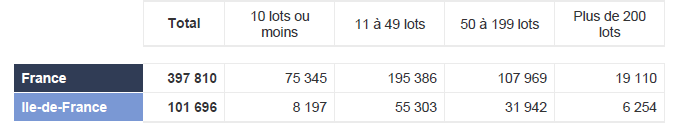
\includegraphics[width=0.7\linewidth]{images/nombreDeCoproprietesParLots}
		\caption[Nombre de copropriétés par lots]{}
		\label{fig:nombredecoproprietesparlots}
	\end{figure}
	
	\begin{figure}[h]
		\centering
		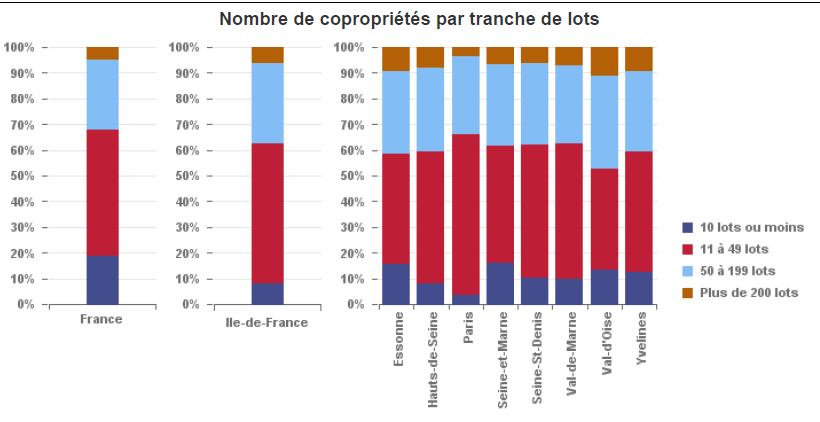
\includegraphics[width=0.7\linewidth]{images/tailleDesCoproprietes}
		\caption[Taille des copropriétés]{Taille des copropriétés (les copropriétés de moins de 10 lots sont sans doute sous représentées)}
		\label{fig:tailledescoproprietes}
	\end{figure}
	
	\subsection{Quels sont les immeubles régis par le statut de la copropriété ?}
	
		\subsubsection{Définition du champ d’application par l’article 1 de la Loi 65-557 du 10 juillet 1965 modifie par l’ordonnance du 30 octobre 2019}
		Les immeubles auxquels s’applique le statut de la copropriété sont désignés à l'article 1er de la loi du 10
		juillet 1965, ainsi rédigé après l’Ordonnance du 30 octobre 2019 :
		\begin{quote}
			« \textsc{i} - La présente loi régit tout immeuble bâti ou groupe d’immeubles bâtis à usage total ou partiel
			d’habitation dont la propriété est répartie par lots entre plusieurs personnes
			Le lot de copropriété comporte obligatoirement une partie privative et une quote-part de parties
			communes, lesquelles sont indissociables. [$\dots$]
			
			« \textsc{ii} - A défaut de convention y dérogeant expressément et mettant en place une organisation dotée de
			la personnalité morale et suffisamment structurée pour assurer la gestion de leurs éléments et services
			communs, la présente loi est également applicable :
			
			« 1\degre{} A tout immeuble ou groupe d’immeubles bâtis à destination totale autre que d’habitation dont la
			propriété est répartie par lots entre plusieurs personnes ;
			
			« 2\degre{} A tout ensemble immobilier qui, outre des terrains, des volumes, des aménagements et des services
			communs, comporte des parcelles ou des volumes, bâtis ou non, faisant l’objet de droits de propriété
			privatifs.
			
			« Pour les immeubles, groupes d’immeubles et ensembles immobiliers mentionnés aux deux alinéas cidessus
			et déjà régis par la présente loi, la convention mentionnée au premier alinéa du présent II est
			adoptée par l’assemblée générale à l’unanimité des voix de tous les copropriétaires composant le
			syndicat. »
		\end{quote}
	
		\subsubsection{Le double champs d’application du texte : Obligatoire ou supplétif}
			Avant l’Ordonnance du 30 octobre 2018, l’article 1 n’était expressément visé parmi les
			dispositions « d’ordre public » du texte.
			
			Cependant, du fait de sa rédaction, les auteurs et la jurisprudence considéraient que l'on ne
			pouvait déroger au statut de la Copropriété dès lors que la propriété de l'immeuble ou du groupe
			d'immeubles est répartie entre plusieurs personnes\footnote{
			Civ 3\degre{} 15 nov. 1989 : Bull. civ. III \no 213 p. 117; D. 1990. J. 195 note Giverdon et Capoulade
			Un immeuble avait fait l'objet d'une donation-partage et à cette occasion avait été établi un État descriptif de division créant plusieurs lots ensuite vendus à des personnes différentes. Mais cet État descriptif de division ne fixait pas de quotes-parts de parties communes attribuées à chaque lot. Un propriétaire ayant réalisé des travaux sur parties communes prétendait que la loi sur la copropriété ne s'appliquait pas du fait que s'il existait des lots, ceux-ci ne comportaient pas de quote-part de parties communes. La cour de cassation répond : << le statut des immeubles bâtis s'applique de plein droit dès que sont remplies les seules conditions prévues à l'article 1er, alinéa 1er, de la loi du 10 juillet 1965 >>.
			Également Civ. 3\degre{} Ch. 30 juin 1998, JCP G. 1998, IV, 2961	
			}, et ce alors même qu'aucun Règlement de Copropriété n'a été établi.
			
			L’ordonnance du 30 octobre 2018 consacre ce caractère d’ordre public, car l’article 1 fait
			désormais partie des textes énumérés par l’article 43 de la Loi 65-557 du 10 juillet 1965, et toute
			clause contraire est « réputée non écrite ».
			
			Toutefois, le champ d’application « obligatoire » est cantonné par le grand (\I) de l’article 1 :
			\begin{itemize}
				\item aux « immeubles ou groupes d’immeuble bâtis dont la propriété est
				repartie par lots comprenant chacun une partie privative et une quote part
				de parties communes, les deux étant indissociables » (il existe une
				indivision forcée sur les parties communes) ;
				\item\textbf{ si ces immeubles sont partiellement à usage d’habitation}, ce qui est une
				nouveauté issue de l’ordonnance
			\end{itemize}
		
			Inversement, le statut peut être écarté par une convention expresse mettant en place une
			personne morale suffisamment structurée (\II) :
			\begin{itemize}
				\item \textbf{pour un ensemble immobilier} (parcelles ou volumes distinct) dans lequel il
				n’y a pas de propriété indivise mais des terrains, volumes, équipements ou
				services « communs », c’est-à-dire d’intérêt collectif
				\item \textbf{même dans un Immeuble ou groupe d’immeuble comportant des parties
				communes en indivision}, si les lots sont tous à usage autre que d’habitation
			\end{itemize}
		
		\subsubsection{Les éléments indifférents à l’application du statut}
		
			\paragraph{L’absence d’organisation}
			
			L’absence d’assemblée générale ou de syndic (absence d’organisation de la copropriété) ne sont pas des
			conditions d’application du statut de la copropriété\footnote{Cass. Civ. 3e 14 décembre 2010 – Juris Data \no 2011-000224}. D’ailleurs, les premières immatriculations de	copropriété révèlent que \pourcent{20} des copropriétés seraient dépourvues de syndic, et ce chiffre est sans doute sous- estimé car l’immatriculation se fait alors au fil des ventes par les notaires
			
			\paragraph{L’absence d’immatriculation}
			
			De même, l’absence d’immatriculation de l’immeuble au Registre des Copropriétés est sans conséquence
			sur l’application du statut (article 1-1 de la Loi 65-557 du 10 juillet 1965 issue de la loi \no 2018-1021 du 23
			novembre 2018 dite ELAN, dernier alinéa).
			
			\paragraph{L’absence de règlement de copropriété}
			
			Lorsqu’un ensemble immobilier fait l’objet d’un état descriptif de division mais qu’il n’y a pas de règlement
			de copropriété, cet immeuble est soumis à la loi du 10 juillet 1965\footnote{Cass. Civ. 3e 1er décembre 2009 pourvoi: 08-22102}. En ce cas, l’état descriptif de division, quelle que soit sa date, approuvé ou non, revêt un caractère contractuel entre colotis (résultant de l’acte de vente) et ses clauses engagent les colotis entre eux pour toutes les stipulations qui y sont contenues\footnote{Cass. Civ. 3e 12 janvier 2011 pourvoi: 09-13822}.
			La vente de lot de copropriété en l’absence de règlement de copropriété et d’état descriptif de division
			n’est pas nulle pour indétermination de l’objet (1109 Code Civil) dès lors que les lots étaient individualisés
			et qu'il n'en résultait aucune confusion avec les lots de l'autre copropriétaire, bien que le règlement de
			copropriété soit obligatoire et doit être soumis à l’acquéreur\footnote{Cass. Civ. 3e 17 novembre 2010}.
	
	\subsection*{Plan}
		Pour déterminer le champ d’application du statut de la copropriété, il faut par conséquent distinguer :
		\begin{itemize}
			\item La copropriété des régimes voisins, dans lesquels il n’existe pas de division de
			l’immeuble entre plusieurs propriétaires ayant des droits concurrents sur les parties
			communes % (section I)
			\item La copropriété horizontale, la copropriété verticale et la construction en volume
			%(section II)
			\item Pour ce qui concerne les ensembles comprenant plusieurs bâtiments, les « groupes
			d’immeubles bâtis », pour lesquels le statut de la copropriété s’applique
			obligatoirement, des « ensembles immobiliers » pour lesquels une organisation
			différente peut être mise en place %(section III)
			\item Enfin, il sera examiné la comptabilité entre le statut de la copropriété et les
			servitudes %(section IV)
		\end{itemize}

\section[Champ d’application impératif]{Champ d’application impératif (article \II) : immeuble ou groupe d’immeuble affecte a l’habitation}
	Depuis l’Ordonnance du 30 octobre 2019, l’article \I{} repose sur une double opposition
	\begin{itemize}
		\item l’Immeuble ou le groupe d’immeuble par opposition à « l’ensemble immobilier »
		\item et l’affectation à usage total ou partiel d’habitation par opposition à l’Immeuble ou le
		groupe d’immeuble à « destination totale autre que d’habitation »
	\end{itemize}
	
	Le champ d’application impératif du statut est désormais le suivant :
	\begin{quote}
		« \I{} - La présente loi régit tout immeuble bâti ou groupe d’immeubles bâtis à usage total ou partiel
		d’habitation dont la propriété est répartie par lots entre plusieurs personnes.
		Le lot de copropriété comporte obligatoirement une partie privative et une quote-part de parties
		communes, lesquelles sont indissociables. »
	\end{quote}
	
	\subsection{L’immeuble ou « groupe d’immeuble bâtis » caractérisé par l’homogénéité du sol}
	
		\subsubsection{Critère de distinction : homogénéité du sol}
		
			Qu'est-ce qui différencie le groupe d'immeubles bâtis où le statut sur la copropriété s'applique
			nécessairement, de l'ensemble immobilier où le statut de la copropriété ne s'applique qu'à défaut de
			conventions contraires ?
			
			Selon l’article 1, c’est l’existence de lots « comportant obligatoirement une partie privative et une
			quote-part de parties communes, lesquelles sont indissociables » qui justifie l’application
			impérative du statut, en d’autres termes la situation d’indivision forcée et perpétuelle dans
			laquelle se trouve les copropriétaires sur les parties communes qui détermine l’application du
			statut impératif.
			
			Cette situation correspond naturellement à un immeuble unique divisé en lots, mais également –-- c’est
			l’hypothèse du « groupe d’immeubles bâtis » aussi appelé « copropriété horizontale » --- à une parcelle
			cadastrale unique sur laquelle sont édifiés plusieurs bâtiments ou pavillon, tant que tous copropriétaires
			ont à la fois des « parties privatives » (appartement ou maison) et des droits indivis dans le sol (partie
			commune).
			
			Par conséquent, le groupe d’immeuble bâti relevant impérativement du statut de la copropriété se
			caractérise par l’homogénéité su sol, par opposition à l’hétérogénéité de la propriété du sol dans un
			ensemble immobilier\footnote{
			Givord, Giverdon, Capoulade, La Copropriété, Ed. Dalloz 2018 p. 85 ; Atias, Guide de la Copropriété bâtie, Edilex, 6\degre{} Edition, p. 35 ;
			Lafond Roux, Code de la Copropriété Ed. 2018 p. 11, J. Cabanac, Les ensembles immobiliers et le nouveau statut de la copropriété : Inf.
			rap. copr. mai 1966, p. 66. – Les ensembles immobiliers et la loi du 10 juillet 1965 : Gaz. Pal. 1966, 1, doctr. p. 117.– B. Leclercq, Les
			ensembles immobiliers : Rapport au 73e Congrès des notaires de France, Strasbourg 1976, p. 403 et s. – C. Lebatteux et J. Barnier-
			Sztabowvicz, Les ensembles immobiliers et l'adoption de l'organisation différente : Administrer juin 1994, p. 9 et s. – P. Capoulade :
			Copropriété et structures foncières dans la jurisprudence de la Cour de cassation : Administrer janv. 1996, p. 4 et s. – P. Capoulade et
			Cl. Giverdon, Propos sur les ensembles immobiliers : RD imm. 1997, p. 161 et s..
			} . Il y a homogénéité lorsque tous les propriétaires ont des droits réels sur
			l'ensemble du terrain servant d'assiette aux immeubles. Comme l’a écrit Pierre CAPOULADE\footnote{Administrer janvier 2001 \no 329 p. 37 et suivantes.} :
			\begin{quote}
				« Les copropriétaires possèdent des droits indivis sur l’ensemble du sol. Ils disposent sur celui-ci d’une
				quote-part numérique entrant, d’une manière indissociable avec les parties privatives, dans la composition
				du lot de copropriété ».
			\end{quote}
	
		\subsubsection{Exemples :}
			\begin{enumerate}
				\item Groupe d’immeuble bâti sur une seule parcelle comportant plusieurs Bâtiments d’habitation ou
				mixte (avec plusieurs lots), et des maisons individuelles chacune constitutive d’un lot, mais le sol
				est indivis
				\begin{center}
					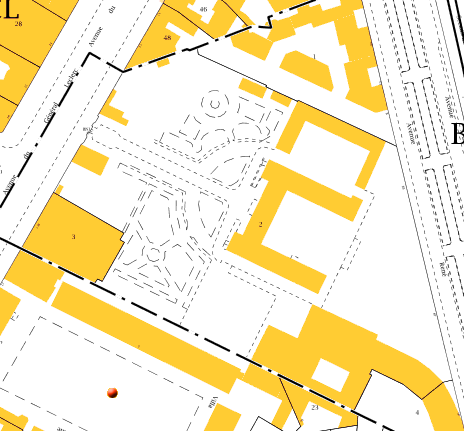
\includegraphics[width=0.7\linewidth]{images/assietteCopro}
				\end{center}
				
				\item  Plan à rez-de-chaussée d’une copropriété (en jaune pâle : parties communes :
				sol et hall), avec deux Bâtiments constitués en lot
				\begin{center}
					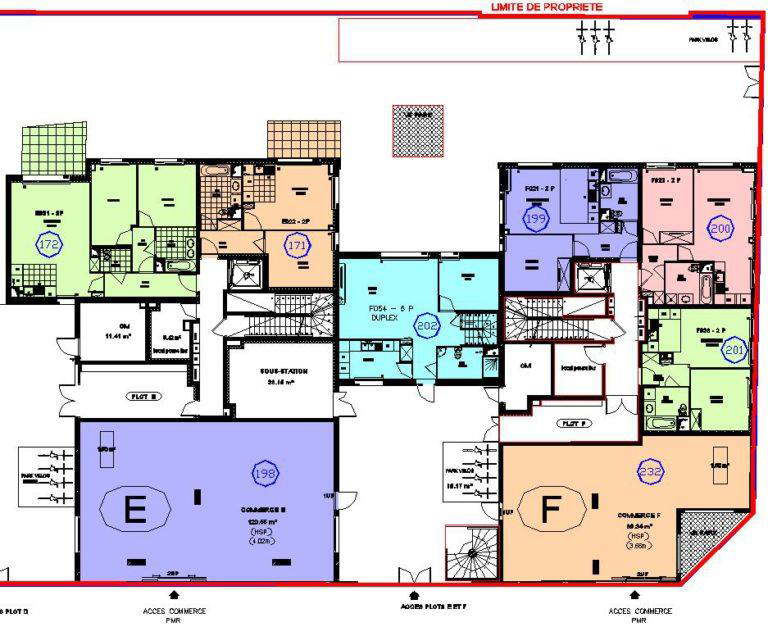
\includegraphics[width=0.7\linewidth]{images/planRdcCopro}
				\end{center}
				
				
				\item Plan de coupe d’une copropriété « verticale » classique
				\begin{center}
					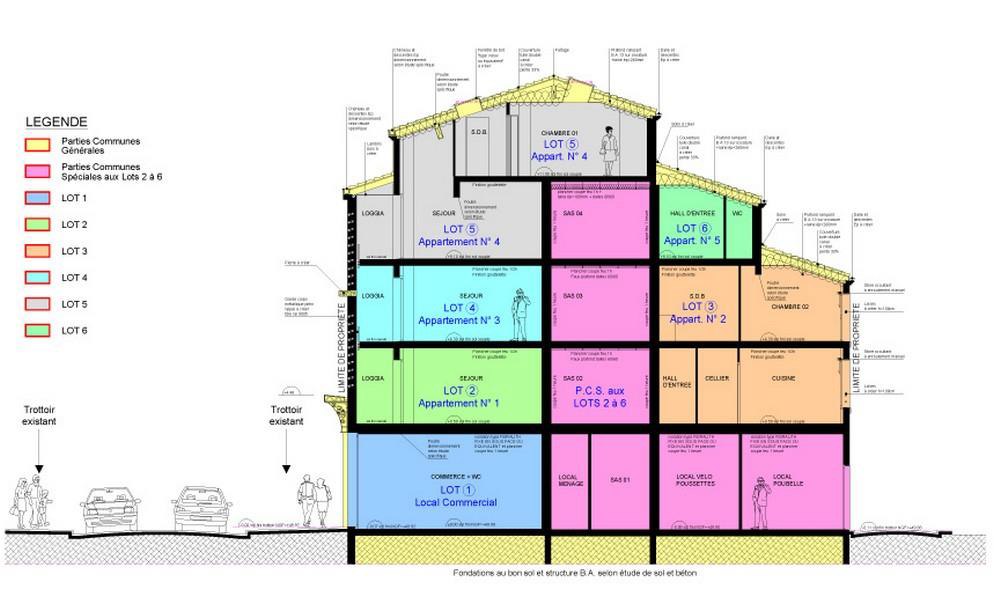
\includegraphics[width=0.7\linewidth]{images/planCoupeCopro}
				\end{center}
				
			\end{enumerate}

		\subsubsection{Conséquences}
			Lorsque la propriété du sol est homogène (appartenant indivisément à l’ensemble des copropriétaires), il
			existe un syndicat des copropriétaires de plein droit. Certes il sera possible de créer des syndicats
			secondaires pour chacun des bâtiments mais il n’y aura toujours qu’un seul syndicat « principal ».
			Ce principe a amené la Cour de Cassation à préciser qu’en cas de division d’un lot donnant vocation à la
			construction d’un bâtiment, la division de ce lot ne peut avoir pour conséquence de créer une seconde
			copropriété sur un terrain homogène\footnote{
			3\degre{} civ. 18 janv. 2018, \no 16-26072 au Bulletin et sur le site de la cour de cassation.
			} quand bien même ce lot correspondrait-il à un bâtiment séparé.
			
			La Cour d'Aix en Provence\footnote{
			16 avril 1992, Résidence l'Esplanade, Loyers et Copropriété 1993.272 et RTDI 93 p 115
			} a également retenu ce critère du régime du sol : retenant que l'immeuble
			présentait une structure homogène, l’arrêt a refusé d'assimiler l'Esplanade à un ensemble immobilier et
			a jugé en conséquence que seul le statut de la Copropriété devait recevoir application. En sorte que sur la
			demande d'un copropriétaire, les décisions de l'association syndicale libre mise en place par le promoteur
			de la Résidence lui ont été déclarées inopposables.
			
	\subsection{L’affectation a « usage total ou partiel d’habitation », nouveau critère du champ d’application impératif}

		Jusqu’à l’ordonnance du 30 octobre 2019, le statut de la copropriété s’appliquait à toutes sortes
		d’immeubles, quel que soit leur destination, dès lors que l’on se trouve en présence du régime homogène
		de la propriété du sol (chaque copropriétaire ayant des droits indivis sur la totalité du sol).
		
		En sorte que le statut s’applique bien évidemment aux immeubles d’habitation comme aux immeubles
		mixtes (habitation, professionnel, bureaux, commerces $\dots$) qui constituent la majorité en nombre
		d’immeubles soumis au statut de la copropriété. Mais le même statut s’applique également
		obligatoirement aux immeubles à usage exclusif de bureaux ou de commerces, et ce quel que soit le mode
		d’exploitation de l’immeuble dès lors que celui-ci se trouve divisé par lots.
		
		L’Ordonnance du 30 octobre 2019 revient aux origines du droit de la copropriété et aux intentions du
		législateur : que ce soit dans l’article 664 du Code civil de 1804 ou dans la loi du 28 juin 1938, les textes
		envisageaient la copropriété sous son aspect « habitation » : rappelons-nous en effet que le statut de la
		copropriété issu de la loi du 28 juin 1938 constituait le titre \II{} de cette loi, dans le titre 1\ier{} régissait les
		sociétés d’attribution qui avaient pour objet l’acquisition d’un appartement sur plan.
		
		La loi de 1965 a eu pour volonté principale d’établir un équilibre dans les droits et devoirs des
		copropriétaires à titre individuel d’une part et à titre collectif d’autre part ; implicitement cet équilibre
		concerne essentiellement les immeubles d’habitation : les travaux préparatoires de la loi de 1965 faisaient
		état de l’avenir « de l’habitat urbain ». Depuis lors s’est développée une conscience consumériste à laquelle
		l’idée du logement n’est pas étrangère. Enfin l’étude d’impact du projet de loi ELAN s’interrogeait
		justement sur la possibilité de différencier le statut selon le type d’occupation de l’immeuble.
		
		On peut s’interroger sur le point de savoir si le statut protecteur de la copropriété doit effectivement
		profiter à des immeubles exclusivement consacrés à des activités professionnelles : qu’il s’agisse de
		commerces ou d’immeubles de bureaux réalisés par des investisseurs.
		
		Le gouvernement a décidé de franchir le pas en modifiant l’alinéa 1er de la loi du 10 juillet 1965 par l’ajout
		des mots « \textit{à usage total ou partiel d’habitation} », en sorte qu’\textit{a contrario }le statut de la copropriété ne s’applique pas de plein droit aux immeubles dont la propriété est répartie par lots entre plusieurs
		personnes dès lors qu’aucun de ces lots n’a vocation à être affecté à l’habitation.
		
		Notons que pourra également échapper au statut de la copropriété un immeuble composé exclusivement
		de parkings !
		
		Cette réduction du champ d’application obligatoire du statut est tellement importante que l’Ordonnance
		a jugé utile de la réaffirmer dans l’alinéa 2 de l’article 1er de la loi en faisant état de la possibilité
		d’échapper au statut de la copropriété lorsqu’il s’agit « \textit{de tout immeuble ou groupes d’immeubles bâtis, à
		destination totale autre que l’habitation} ».
		Ainsi, le statut de la copropriété « obligatoire » est écarté, \textbf{alors même que l’immeuble est divisé par lots
		et que le sol est homogène, dès lors qu’il n’y a aucun lot à usage d’habitation}.
	
		Toutefois, l’affectation d’un sol lot à usage d’habitation (loge de gardien par exemple), aura pour
		conséquence de faire retomber l’immeuble en copropriété.

\section{Le champ d’application supplétif du statut : les ensembles immobiliers et les immeubles a destination autre que d'habitation}
	Le champ d’application du statut « par subsidiarité » (à défaut d’organisation contraire), ou supplétif est
	désormais défini, en application de l’article 1-\II{} de la Loi 65-557 du 10 juillet 1965 dans sa rédaction issue
	de l’Ordonnance du 30 octobre 2019
	\begin{quote}
		« \II. - A défaut de convention y dérogeant expressément et mettant en place une organisation dotée de
		la personnalité morale et suffisamment structurée pour assurer la gestion de leurs éléments et services
		communs, la présente loi est également applicable :
		« 1\degre{} A tout immeuble ou groupe d’immeubles bâtis à destination totale autre que d’habitation dont la
		propriété est répartie par lots entre plusieurs personnes ;
		« 2\degre{} A tout ensemble immobilier qui, outre des terrains, des volumes, des aménagements et des services
		communs, comporte des parcelles ou des volumes, bâtis ou non, faisant l’objet de droits de propriété
		privatifs.
		« Pour les immeubles, groupes d’immeubles et ensembles immobiliers mentionnés aux deux alinéas ci dessus
		et déjà régis par la présente loi, la convention mentionnée au premier alinéa du présent \II{} est
		adoptée par l’assemblée générale à l’unanimité des voix de tous les copropriétaires composant le
		syndicat. »
	\end{quote}
	
	\subsection{Les ensembles immobiliers hétérogènes}
	
		Qu'est ce qu'un ensemble immobilier ? C'est un ensemble dans lequel il existe à la fois :
		\begin{itemize}
			\item Des biens ou services « communs »: terrains, des volumes, des aménagements et des services
			communs, tels par exemple des allées et voies de desserte, un local social, des terrains de jeux
			et de sport, une piscine, des tennis, un gardiennage avec une maison de gardien, etc.
			\item Des parcelles ou volumes, bâtis ou non, faisant l’objet de droits de propriété « privatifs » ou
			« divis » (le sol de ces parcelles n’est pas en indivision forcée).
		\end{itemize}
		
		\subsubsection{L’ensemble immobilier caractérisé par « l’hétérogénéité du sol »}
			Il y a hétérogénéité lorsque l'ensemble immobilier comporte les terrains attribués à différentes personnes
			(le foncier est éclaté), aucune ne pouvant se prévaloir de droits réels (indivis) sur l'ensemble des terrains.
			Mais entre ces différentes parcelles existent des terrains communs, ou des éléments fédérateurs (indivis
			ou non)
		
			M \nom{SIZAIRE} : « à côté d'un terrain et d'éléments communs ou bien superposés à ceux-ci, il existe des propriétés ou des	copropriétés particulières : l'ensemble immobilier est juridiquement hétérogène »\footnote{
			Journées d'étude du CNEIL 22/23 nov. 1965, p. 52}
			
			M \nom{VIGNERON} : « l’ensemble immobilier tient sa spécificité du fait que les sols d’assiette font l’objet de modes d’appropriation différents, en propriété ou en copropriété selon les parcelles incluses dans cet ensemble et autonomes les unes par rapport aux autres »\footnote{
			(G. Vigneron- JurisClasseur Construction - Urbanisme > Fasc. 90-20 : STATUT DE LA COPROPRIÉTÉ. – Champ
			d'application du statut, \no 35}
			
			\paragraph{Exemples}
			
			\subparagraph{Lotissement} : toutes les parcelles font l’objet d’un droit de propriété exclusif, mais il existe des terrains, voiries, équipements d’intérêt collectifs dont la propriété est confiée à une ASL (voie = parcelle cadastrale)
			\begin{center}
				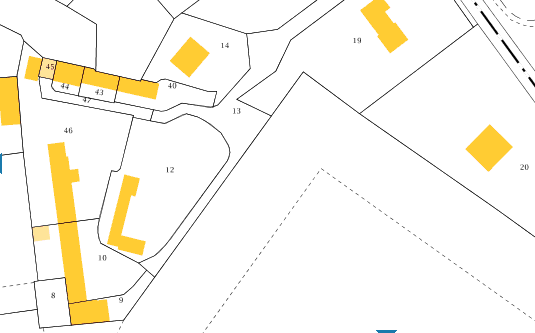
\includegraphics[width=0.7\linewidth]{images/lotissement}
			\end{center}
			
			
			\subparagraph{Voie privée} : Voie laissée en indivision avec de part et d’autres des parcelles distinctes, ou encore faisant l’objet d’une propriété de chaque riverain au droit de sa façade, jusqu’à la moitié de la voie.
			\begin{center}
				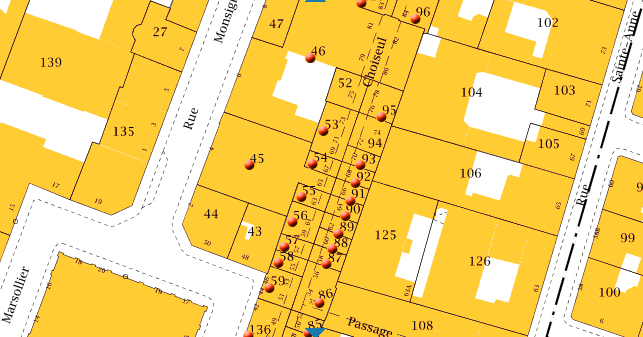
\includegraphics[width=0.7\linewidth]{images/voiePrivee}
			\end{center}
			
		
			\subparagraph{Jurisprudence antérieure à l’ordonnance}
			\begin{description}
				\item[Civ. 3ème 17 février 1999\footnote{Cour de cassation Chambre civile 3 17 Février 1999 \no 97-14.368 Bull. Association foncière urbaine libre Grand Ecran c/ associationsyndicale Italie-Vandrezanne}] : l’ensemble immobilier susceptible de faire l’objet d’une organisation différente résulte du seul fait que certains copropriétaires avaient des droits réels exclusifs sur certaines parcelles du terrain faisant ressortir l’hétérogénéité du régime juridique des fractions de l’ensemble en question.
				
				\item[Civ. 15 décembre 1993\footnote{Civ 15 décembre 1993, pourvoi: 91-12645 , au bulletin, Recueil Dalloz 1994, Somm. p. 205 (Domaine des Clausonnes)}]	: << \textit{Un lotissement comportant, selon les dispositions de l'art. R. 315-1 c. urb., division du sol en propriété ou en jouissance, privant les allotis de droits concurrents sur l'ensemble du terrain, une cour d'appel, qui constate, par motifs non critiqués, qu'un arrêté préfectoral a autorisé le lotissement et approuvé le cahier des charges et qu'une association syndicale a été constituée, d'où il résulte que l'application de la loi \no 65-557 du 10 juill. 1965 se trouve exclue, n'a pas à procéder à une recherche que ses constatations rendaient inopérante et qui n'était pas demandée} >>.
			
				\item[Paris 23\degre{} Ch 29 octobre 1997\footnote{Paris 23\degre{} Ch 29 octobre 1997 Tour Cantate Loyers et Copropriété 1998 \no 20}] Constitue un ensemble immobilier la juxtaposition d’immeubles en copropriété et d’immeubles	appartenant à une société détentrice de droits réels exclusifs sur une partie du terrain.
			\end{description}
		
		\subsubsection{L’ensemble immobilier dit « complexe » (en volumes)}
		
			\paragraph{Origine}
			
				La loi sur la copropriété ne s'applique pas nécessairement à des locaux superposés ou imbriqués, sans
				création corrélative de parties communes.
				En effet, il existe une présomption posée par l'article 552 du Code Civil, selon laquelle << la propriété du sol
				emporte la propriété du dessus et du dessous >> ; mais la preuve contraire peut être rapportée : c'est le cas
				assez fréquent d'une cave qui déborde sur le terrain voisin. Cette cave << débordante >> ne sera pas en
				copropriété avec l'immeuble dans le sol duquel elle se trouve.\footnote{
				Civ 1\degre{}, 2 avril 1962. B. \no 66, p. 54; cf également Civ 3\degre{} 11 mai 1994 RD Imm 1994, 486 pour une terrasse qui constitue
				le sol d'un immeuble et la couverture d'un autre immeuble.}
				
				La généralisation de ce mécanisme a permis la création de construction dites en « volume » (ou Ensembles
				Immobiliers Complexes) qui échappent également au statut de la copropriété.
				
				<< \emph{La volonté de limiter le gaspillage de l'espace se concrétisa avec l'apparition d'un nouveau parti
				architectural et urbanistique : << \emph{l'ensemble immobilier complexe (E.I.C.)} >>, ouvrage formant un tout,
				techniquement indivisible, où se juxtaposent, se superposent, s'imbriquent, s'articulent des volumes de
				destinations variées (habitations, activités, équipements, circulation, etc) et où l'utilisation systématique
				du tréfonds fait disparaître la notion même de sol naturel. L'objectif consiste à aménager non plus des
				terrains, mais l'espace urbain dans ses trois dimensions} >>(\nom{Walet} et \nom{Chambelland})\footnote{
				Walet et Chambelland in La Construction en Volumes (Masson Editeur, 1989)}
				
			\paragraph{Définition}
				Selon MM \nom{Walet} et \nom{Chambelland}, l'E.I.C. sera caractérisé :
				\begin{quote}
					<< 1\degre{} Par la juxtaposition et la superposition à l'intérieur \emph{d'une même structure technique},
					de volumes dont chacun \emph{abrite une fonction spécifique} et reçoit un statut \emph{approprié à
					celle-ci} ;
					<< 2\degre{} par son absence de parties communes entre ces volumes, \emph{absence due à
					l'hétérogénéité juridique de ces derniers} ;
					<< 3\degre{} par son appropriation, sa construction, sa gestion par \emph{deux ou plusieurs maîtres
					d'ouvrage} dont souvent l'un d'eux \emph{relève du droit public} ;
					<< 4\degre{} par ses contraintes de construction et de gestion entraînées à la fois par la structure
					technique et la pluralité de maîtrises de l'ouvrage et de destinations;
					<< 5\degre{} par l'intervention d'un spécialiste, promoteur ou aménageur. >>
				\end{quote}
			
				\begin{figure}[h]
					\centering
					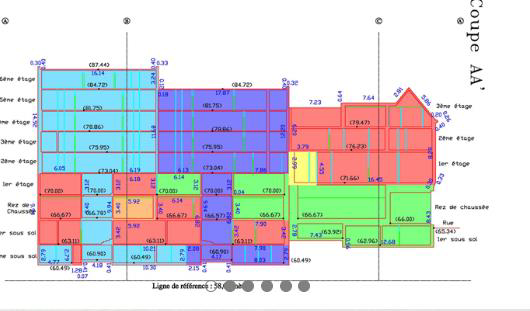
\includegraphics[width=0.7\linewidth]{images/volumetrieCoupe}
					\caption[Exemple : Urbanisme sur Dalle (Nanterre)]{}
					\label{fig:volumetriecoupe}
				\end{figure}
				)
				Le plus souvent on trouve à l’origine de cette conception :
				\begin{itemize}
					\item une dalle servant de base à l'aménagement d'une zone --- cette dalle sera un ouvrage public;
					\item  plusieurs niveaux techniques et à usage de parkings sous la dalle ;
					\item des ouvrages ou parties d'ouvrages à vocation publique également (service de mairie
					ou Tribunal de commerce par exemple à Nanterre) sur la dalle ; 
					\item  à côté de ces ouvrages à caractère public ou parfois même au-dessus on trouvera des commerces
					et des habitations.
				\end{itemize}
				
				Chaque volume sera défini en altimétrie par rapport au Nivellement Général de la France\footnote{
				Une altitude est un écart de hauteur par rapport à un niveau de référence, le niveau moyen des mers. En France, l’altitude 0 correspond au niveau moyen de la Méditerranée enregistré au marégraphe de Marseille (dans le Vieux Port) de 1885 à 1897.
				Depuis ce lieu les géomètres ont parcouru l’Hexagone pour installer des repères d’altitude par la méthode du nivellement	géométrique précis à quelques millimètres. Il y a actuellement 450.000 repères sur un réseau de \nombre{300 000} kms de long.
				}(NGF) en sorte que la propriété du volume sera comprise entre deux cotes N.G.F.
				
				A l'intérieur du volume pourront être créés plusieurs niveaux qui seront eux-mêmes soumis à un statut
				prédéterminé, par exemple le volume A sera une propriété unique (Un Commerce au niveau O) et le
				volume B une copropriété (habitations du niveau 1 au niveau 5).
				
				S'il n'existe pas de parties communes, il existe cependant une certaine imbrication entre les différents
				volumes. Ces imbrications feront l'objet de servitudes entre les volumes (servitude d'appui, d'accrochage,
				de vue, etc ...).
				
				Il n’y a pas de copropriété s’il n’y a pas de parties indivises entre les copropriétaires (parties communes)\footnote{
				Cass. Civ 3e 8 septembre 2010
				}. Ces volumes seront le plus souvent regroupés en une Association Syndicale de Propriétaires qui gérera
				l'Ensemble Immobilier.
				
			\paragraph{Volumétrie par « affectation »}
				On peut s'interroger sur la légalité d'un découpage de bâtiments qui ne correspond pas à une réalité
				physique. Mais on imagine mal les tribunaux remettre en cause un nombre aujourd'hui important
				d'opérations immobilières d'envergure\footnote{
				Sur la question Cf. Sizaire - Division en volumes et Copropriété des immeubles bâtis JCP 88.1.3367.
				}
				
				Étant toutefois observé l'abus manifeste de certains promoteurs qui pour mieux vendre certains locaux en
				les faisant échapper aux contraintes de la loi de 1965 n'hésitent pas à créer des Divisions en volumes
				purement artificiels qui comprennent deux parties : un volume commercial au rez de chaussée et un
				volume habitation pour les étages au-dessus des commerces.
				
				La loi ALUR a consacré l’organisation des immeubles en volumes… dans l’hypothèse de la scission d’une
				copropriété initiale devant donner naissance à plusieurs propriétés distinctes. L’article 28 de la loi sur la
				scission comporte désormais deux nouveaux paragraphes qui sont ainsi rédigés :
				\begin{quote}
					\textsc{iv}. – La procédure (de scission) prévue au présent article peut également être employée pour la
					division en volumes d’un ensemble immobilier complexe comportant soit plusieurs bâtiments
					distincts sur dalle, soit plusieurs entités homogènes affectées à des usages différents pour autant
					que chacune de ces entités permettent une gestion autonome. Si le représentant de l'État dans le
					département ne se prononce dans les deux mois, son avis est réputé favorable.
					
					Elle ne peut en aucun cas être employée pour la division en volumes d’un bâtiment unique. ($\dots$)
				\end{quote}
			
				Toutefois il convient d’observer qu’en excluant la division en volumes d’un bâtiment unique, le législateur
				semble considérer que la Volumétrie doit correspondre à une « autonomie de gestion ».
				
			\paragraph{Consécration par l’ordonnance du 30 octobre 2019}
				
				L’ordonnance du 30 octobre 2019 a consacré la possibilité de constituer un Ensemble Immobilier
				complexe, puisque l’article 1- \II{} vise explicitement l’hypothèse de l’ensemble immobilier composé non de
				« parcelles » mais de « volumes ».
				
				Contrairement à ce qui avait été pressenti, l’ordonnance ne restreint pas les cas dans lesquels une mise
				en Volume est envisageable, par exemple en exigeant une autonomie structurelle ou une superposition
				des domaines publics et des domaines privées. Elle se contente de renforcer les exigences concernant
				l’organisation à mettre en place pour éviter à ces ensembles de se trouver « sans gouvernail », mais ces
				exigences ne sont pas de nature à éviter certains abus ( par exemple, la prise en charge de la toiture
				exclusivement par le volume supérieur, qui se trouve être celui d’habitation).
				
				Aussi, l’ordonnance pourrait-elle avoir un effet accélérateur sur la constitution d’ensembles immobiliers
				en Volumes :
				\begin{itemize}
					\item  elle supprime le contrôle du Préfet (prévu dans la loi \no 2014-366 DU 24 MARS 2014 DITE ALUR)
					en cas de scission en Volumes
					\item  elle encourage le découpage d’un ensemble Immobilier complexe en volumes « par
					affectation », dès lors que le Volume « commerce » en pied d’immeuble, même s’il est lui-même
					divisé en plusieurs lots comportant des parties communes indivises, pourra échapper
					complètement au statut de la copropriété
				\end{itemize}
		
		\subsubsection{Les éléments fédérateurs}
			Pour être qualifié comme tel, l’ensemble immobilier doit cependant nécessairement comprendre un ou
			des éléments fédérateurs, constitués par « \emph{des terrains, des volumes, des aménagements et des services communs} » tels que, par exemple, des parcelles indivises, une impasse commune\footnote{3ème Civ., 11 février 2009, Bull. civ., III, \no 34, pourvoi 08-10109}, une chaufferie
			centrale\footnote{3ème Civ., 21 juin 2000, pourvoi \no 98-20897}, etc.
			Ces « choses communes » peuvent être en indivision forcée, attribuées de façon divise à chaque coloti (
			voie privée propriété de chaque coloti jusqu’à la moitié de la voie) ou leur propriété peut être transférée
			à l’organisme de gestion ( à l’ASL en lotissement)
			La question qui peut se poser est celle de savoir si des aménagements communs, en l’absence de terrain
			commun suffisent à constituer un ensemble immobilier : en effet l’énumération de l’article 1 – II de la loi
			issu de l’ordonnance (et avant de dernier alinéa de l’article 1) et reliée par la conjonction « et », et non ou
			Cela signifie-t’il qu’il faut « en plus » de terrains ou volumes communs, des aménagements ou des
			équipements communs ? En l’état de la jurisprudence il semble qu’il suffit d’avoir un élément commun
			pour constituer un ensemble immobilier\footnote{
			(Civ. 3\degre{} Ch. 21 juin 2000, Pourvoi \no 98-20897) – Solution critiquée par Atias ; op. cit. p. 35
			}	(par exemple une chaufferie commune).
	
	\subsection{Les ensembles immobiliers à destination autre que d’habitation (ordonnance du 30 octobre 2019)}
		Relèvent également du champ supplétif d’application de la copropropriété « tout immeuble ou groupe
		d’immeubles bâtis à destination totale autre que d’habitation dont la propriété est répartie par lots entre
		plusieurs personne »
		
		Il faut noter que les termes du \I{} et du \II{} ne sont pas totalement transposable : le \I{} (champ d’application
		obligatoire) parle des immeubles « à usage total ou partiel d’habitation », tandis que le \II{} (champ
		d’application supplétif) parle des immeubles « à destination autre que d’habitation ».
		
		Or, en principe, la destination résulte du règlement de copropriété, et elle est intangible, tandis que l’usage
		d’un lot est une question de fait, un lot pouvant librement changer d’usage (ou d’affectation), tant que ce
		changement demeure compatible avec la destination de l’immeuble.
		
		En réalité, ces deux conditions sont sans doute cumulatives. Pour qu’un immeuble puisse être soumis à un
		statut autre que la copropriété :
		\begin{itemize}
			\item il faut qu’à sa conception, donc dans le « cahier des charges » constitutif, il se trouve
				intégralement destiné à un usage autre que d’habitation ;
			\item il faut en outre que cette destination ait été respectée concrètement, car si l’immeuble devient
				à usage partiel ou total d’habitation, il retombera sous le coup du statut de la copropriété.
		\end{itemize}
	
	\subsection{L’exigence d’une organisation différente « suffisamment structurée » et « dotée de la personnalité morale » (ordonnance du 30 octobre 2019)}
		Bien que l’ordonnance ait pour l’essentiel consacré l’évolution jurisprudentielle en cours, elle crée pour
		ces immeubles soumis à un statut « alternatif » à la copropriété un cadre beaucoup plus rigide que celui
		de l’ancien article I dernier alinéa qui se contentait d’appliquer le statut aux ensembles immobiliers
		hétérogènes « à défaut de convention contraire créant une organisation différente ».
		
		Désormais, le statut redeviendra applicable « à défaut de \emph{convention y dérogeant expressément} et mettant
		en place une organisation dotée de la \emph{personnalité morale} et \emph{suffisamment structurée pour assurer}, la
		gestion de leurs éléments et services communs, la présente loi est également applicable ($\dots$) ».
		
		\subsubsection{Exigence d’une dérogation explicite}
			L’Ordonnance substitue au mot « convention contraire » les mots « convention y dérogeant
			expressément ». Ce faisant le texte reprend purement et simplement les mots qui avaient été retenus
			dans l’arrêt de la cour de cassation du 19 septembre 2012.
			
			Cette modification est heureuse : la convention à intervenir n’est pas nécessairement contraire aux
			dispositions de la loi de 1965 ; on peut concevoir en effet la mise en place d’une ASL qui outre les quelques
			dispositions impératives de l’Ordonnance du 1er juillet 2004, reprendrait pour l’essentiel les dispositions
			de la Loi 65-557 du 10 juillet 1965, par exemple quant à la répartition des charges.
		
		\subsubsection{Exigence de la création d’une personne morale}
		
			Cette précision est une codification de la jurisprudence récente de la Cour de Cassation. En effet, certaines
			voies privées, ou certains lotissements (avant 1943) sont dotés d’un cahier des charges, ou d’une
			convention d’indivision ou de servitude, indiquant les modalités de répartition des charges, voire de prise
			de décision, mais dépourvus de la personnalité morale, si bien qu’ils constituent des groupements de fait\footnote{cf. civ. 3\degre{} Ch. 31 mars 1993 \no 90-10143.}.
			
			Cette situation aboutit immanquablement à une impasse : dépourvu des attributs de la personnalité
			morale, un tel groupement ne peut ni régulariser de contrat, ni agir en justice pour préserver les
			« éléments fédérateurs », ni poursuivre judiciairement l’un de ses membres en recouvrement des charges.
			
			Aussi la cour de cassation\footnote{Civ. 3\degre{} Ch. 19 sep 2012, Pourvoi \no 11-13679 11-13789, au Bulletin} dans un arrêt du 19 septembre 2012 rendu à propos d’immeubles divisés en
			volumes, avait-elle déjà considéré que le statut ne pouvait être écarté en l’absence de personnalité
			juridique assurant l’entretien de ces éléments d’équipement:
			\begin{quote}
				« Attendu que, pour débouter la SCI [\emph{de sa demande tendant à l’application du statut de la
				copropriété}], l'arrêt [$\dots$] relève que l'état descriptif de division stipule que l'ensemble immobilier ne
				sera pas régi par la loi du 10 juillet 1965 et qu'à cette fin, l'acte identifie des volumes immobiliers de
				pleine propriété dans le cadre du régime du droit de superficie, et énonce l'ensemble des servitudes
				issues de l'imbrication de ces volumes qui permettent leur coexistence ainsi que l'attribution [de]
				\nombre{3 026}/\nombre{10 000}\iemes{} des charges générales au lot \no 4, retient que l'état descriptif de division constitue,
				relativement à ce lot, la convention contraire visée à l'article 1er, alinéa 2, de la loi du 10 juillet 1965 ;
				Qu'en statuant ainsi, sans constater la création d'une organisation différente, au sens de la loi, pour
				la gestion des éléments communs de l'ensemble immobilier, la cour d'appel a violé le texte susvisé »
			\end{quote}
		
		\subsubsection{Une personnalité morale « suffisamment structurée » -- les 3 types de	« structures » communément envisageables}
		
		On ignore pour quelles raisons l’Ordonnance a cru devoir exiger que cette personnalité morale soit
		suffisamment structurée.
		
		Si l’on prend cet exemple de l’association syndicale libre l’Ordonnance du 1er juillet 2004 édicte en son
		article 7 que « les statuts fixent son objet, son siège et ses règles de fonctionnement, précise ses modalités
		de financement et le mode de ($\dots$) recouvrement des cotisations ». Aux termes de l’article 9 de la même
		ordonnance du 1er juillet 2004 : l’association « est administrée par un syndicat composé de membres élus
		($\dots$) » et « le syndicat règle par ses délibérations les affaires de l’association ».
		
		Il est vrai cependant que les statuts peuvent être mal rédigés ou contradictoires, mais en ce cas on voit
		mal le juge requalifier l’association syndicale en syndicat de copropriété puisqu’il doit simplement
		appliquer les dispositions du droit des obligations en ce qui concerne l’interprétation des contrats : article
		1188 et suivants modifiés par l’Ordonnance \no 2016-131 du 10 février 2016.
		
		De plus, il a été jugé à maintes reprises qu'un statut d'organisation différente est exclusif du statut de la
		Copropriété : les charges seront réparties conformément aux statuts qui pourront retenir une répartition
		différente de celle organisée par la loi de 1965 (sauf dans l'hypothèse de la Société d'Attribution non
		encore dissoute) : la loi du 10 juillet 1965 est étrangère au fonctionnement d'une ASL régie par
		l’ordonnance du 1er juillet 2004 relative aux associations de propriétaires (ayant remplacé la loi du 21 juin
		1865 abrogée).
		
		Pour autant on peut cependant envisager l’hypothèse où les statuts seraient muets sur des points
		essentiels comme par exemple la majorité applicable aux décisions ou l’absence de répartition des
		cotisations entre les immeubles membres de l’association syndicale libre.
		
		En cette hypothèse et dans le premier cas (absence de mention sur les majorités applicables) le juge devra t-il faire application de la règle de l’unanimité ou pourrait-il requalifier le statut de l’ensemble immobilier
		pour le soumettre au droit de la copropriété ? Dans le second cas (absence de répartition des cotisations),
		on pourrait concevoir effectivement que le juge considère qu’il y a lieu d’appliquer le statut de la
		copropriété. En ce cas il y aurait substitution pure et simple du régime de la copropriété aux statuts de
		l’association syndicale libre.
		
		Face à cette exigence, il sera préférable, de retenir, pour administrer l’immeuble, une des formes
		communément admises pour la gestion des ensembles immobiliers.
		
		\paragraph{L'association de propriétaires de l’ordonnance du 1er juillet 2004 et le décret du 8 mai 2006}
			Ces associations de propriétaires sont en fait les anciennes associations syndicales de la loi du 21 juin 1865.
			L’association de propriétaires peut être libre ou autorisée. La forme moderne de ces Associations est
			l’Association Foncière Urbaine Libre (AFUL), prévue par le Code de l’Urbanisme pour gérer les lotissements
			(art Article L322-9-1 du Code de l’Urbanisme).
			
			La contrainte majeure concernant ces Associations Syndicales est qu’il faut recueillir le consentement
			individuel de tous les membres situés dans son périmètre. L’ASL n’est donc, le plus souvent, que constituée
			\emph{ab initio}. Sinon, l’unanimité est requise.
			
			Ces Associations Syndicales sont administrées par un « Syndicat » élu par l'Assemblée des syndicataires et
			représenté par un Président (salarié ou élu) qui est l'agent d'exécution du Syndicat. Lorsqu’elles
			comprennent des copropriétés, celles-ci peuvent être représentées à l’assemblée générale par le
			président du conseil syndical (ASL) ou le syndic (AFUL), préalablement habilité par l’assemblée générale
			de copropriété.
			
			L’Ordonnance du 1er juillet 2004 et son décret d’application imposent un contenu minimum aux statuts,
			mais ne comprennent pratiquement aucune disposition d’ordre public, ce qui laisse une grande latitude
			dans l’organisation de l’ensemble immobilier.
	
			Toutefois on peut s’inquiéter de cette trop grande liberté s’agissant notamment de la participation aux
			charges qui peut être particulièrement déséquilibrée : par exemple dans un centre commercial où
			l’opérateur pourra avoir tendance à favoriser les « locomotives » - dont les murs peuvent appartenir à une
			ou plusieurs de ses filiales - au détriment des simples « wagons » que sont les boutiques installées le long
			du mail commercial !
			
			De la même façon, les propriétaires minoritaires ne pourront en cas de décision majoritaire contraire à
			leurs intérêts invoquer l’atteinte à la destination de l’immeuble, garde-fou essentiel dans l’application du
			statut de la copropriété.
			
			Il est vrai que le même risque peut exister dans le cas d’ensembles immobiliers à vocation mixte
			(habitation, commerce, bureau). Toutefois le risque est alors limité puisqu’il ne portera que sur les
			éléments fédérateurs à plusieurs immeubles, alors que s’agissant d’un même immeuble à usage exclusif
			de bureaux et/ou de commerces, ce statut (organisation dotée de la personnalité morale et suffisamment
			structurée) s’appliquera à toutes les parties communes.
		
		\paragraph{La Société Immobilière de Gestion et d'Entretien}
		
			Souvent appelée société de location, cette société loue des immeubles ou les met à disposition de ses
			associés. Ce type de société est régi par le droit commun (article 1844 et s. du code civil).
		
		\paragraph{L'Union de syndicats de copropriétaires}
		
			C’est une organisation différente prévue à l’article 29 de la loi de 1965 et qui fait l’objet des articles 63 à
			63-4 du Décret de 1967.
			
			Par exemple, l'ensemble réalisé à la Plagne en Savoie a adopté ce schéma juridique. Notons cependant que
			pour qu'il y ait Union de Syndicats, il faut par application de la loi du 10 juillet 1965 sur la copropriété que
			cette Union comprenne au moins un syndicat de copropriété, peu importe le statut juridique des autres
			immeubles. De plus, cette structure n’est pas juridiquement stable : sauf pour les Unions issues d’une
			scission volumétrique, il ne peut être imposé à l’un des membres de l’union l’interdiction de s’en retirer.
			
			Il n’en reste pas moins que l’Union est une bonne solution pour « recouvrir » d’une personnalité juridique
			une convention de gestion qui en était jusqu’alors dépourvue, car l’adhésion de la copropriété sera votée
			à la majorité de l’article 25 (l’unanimité n’est donc pas requise).
	
	\subsection{Le passage du statut impératif au statut supplétif (et inversement)}
	
		\subsubsection{Modalité de la « sortie » du régime de la copropriété (Ord. 30 oct. 2019)}
		
			L’ordonnance prévoit les modalités selon lesquelles un immeuble déjà existant, pour lequel l’application
			du statut n’est pas ou plus obligatoire, mais qui en relèverait actuellement, pourrait se soustraire au statut
			impératif : il est exigé une décision prise à l’unanimité des copropriétaires.
		
			Bien que le dernier alinéa vise les « deux alinéas ci –dessus », donc tant l’hypothèse d’un immeuble
			pouvant échapper au statut du fait de sa destination autre que d’habitation, que celle d’un ensemble
			immobilier :
			\begin{itemize}
				\item  pour l’immeuble à destination autre que d’habitation, il est normal qu’un changement des
				règles du jeu aussi fondamental relève de l’unanimité des membres du syndicat des
				copropriétaires
				\item  toutefois, pour les ensembles immobiliers hétérogènes, soumis par « défaut » au statut de la
				copropriété, la solution peut s’avérer en contradiction avec les dispositions concernant les
				Unions de Syndicat. En effet, la constitution d’une Union devrait permettre d’échapper au
				statut de la Loi 65-557 du 10 juillet 1965, et ne requière qu’une décision à l’article 25. A moins
				que le gouvernement n’ait considéré que les Unions relevaient encore du statut ?
			\end{itemize}
			
			Par ailleurs, l’adoption de cette convention n’est pas nécessairement incompatible avec le maintien d’une
			indivision forcée sur les parties communes. Pour un immeuble de bureau, par exemple, il pourrait être
			constituée (à l’unanimité) une ASL pour l’administration des parties communes, chacun demeurant
			propriétaire de « lots » comportant une quote part indivise de parties communes. En effet, la division en
			Volumes a posteriori d’un tel immeuble serait sans doute d’une complexité inextricable.
		
		\subsubsection{Exemple de requalification : application du statut de la copropriété aux voies privées dépourvues d’organisation collective}
			
			On peut s'interroger sur la possibilité de faire appliquer la loi aux immeubles riverains d'une voie privée
			lorsque cette voie ne bénéficie pas d'un statut conventionnel (A.S.L.) ou forcé (loi sur l'assainissement de
			1912, aujourd’hui abrogée).\footnote{
			Cf D. \nom{SIZAIRE} Gazette du Palais 14 juillet 1985 p. 4 : Le statut de la copropriété des immeubles bâtis et la gestion des voies privées, cours ou jardins}
			
			Un premier arrêt de cassation, concernant le Passage de Briare\footnote{
			Civ.3ème 11 octobre 2000, \no 99-10039, Administrer janvier 2001 \no 329, comm Capoulade
			}, avait consacré ce principe, étant précisé que la propriété du sol était commune à l’ensemble des immeubles riverains. La cour d’appel avait écarté	l’application de la loi sur la copropriété puisque cette voie était bordée de propriétés distinctes. L’arrêt est cassé car « cette situation n’exclut pas de plein droit l’application du statut de la copropriété pour l’entretien, la gestion et l’administration de la voie. »
			
			La même solution a été retenue sans équivoque dans un arrêt de cassation de la 3ème Chambre de la Cour
			de Cassation du 11 février 2009\footnote{
			Cour de cassation, chambre civile 3, 11 février 2009, \no de pourvoi: 08-10109 Publié au bulletin Cassation Recueil Dalloz,
			\no 8, 26 février 2009, Actualité jurisprudentielle, p.496-497, note Yves Rouquet (“Etablissement d’enseignement et propriété
			commerciale”). Voir également la revue Loyers et copropriété, \no 4, avril 2009, commentaire \no 99, p.23-24, note Guy Vigneron
			(“Ensemble immobilier”).
			}	: la cour d’appel avait considéré que « la copropriété pure et simple
			appliquée à un ensemble immobilier n’est pas sans inconvénient et qu’il existe d’autres modes
			d’organisation différente ». La cassation se fait au visa de l’article 1er alinéa 2 (devenu l’article I-2\degre{}) de la
			loi et avec l’attendu de principe : « Attendu qu'à défaut de convention contraire créant une organisation
			différente, la présente loi est également applicable aux ensembles immobiliers qui, outre des terrains, des
			aménagements et des services communs, comportent des parcelles, bâties ou non, faisant l'objet de droits
			de propriété privatifs ».

\section{Copropriété et autres formes d’appropriation des biens}
	
	\subsection{Copropriété et monopropriété}
	
		La loi sur la copropriété ne s'applique pas lorsqu'une même personne, une même famille ou une même
		société est propriétaire de la totalité de l'immeuble (Cf. les immeubles de rapport du début du siècle).
		
		Mais dès que cette personne (pour payer le ravalement ou pour mettre l'immeuble aux normes de
		salubrité et de confort, par exemple) vend un seul appartement sur l'ensemble de ceux qui composent le
		bâtiment, le statut sur la copropriété reçoit application : par le fait de cette vente la propriété est répartie
		entre plusieurs personnes"\footnote{Civ 1ère 19 janvier 1960. Bull. \no 35 p 28}.
		
		\paragraph{Sur l’apparition de la copropriété}
		Dès lors que la propriété de l'immeuble est répartie entre plusieurs personnes, par lots comportant chacun
		une partie privative constituée d'une maison et une quote-part de parties communes, il y a lieu d'en
		déduire que le statut de la copropriété était applicable à la date où l'immeuble avait comporté deux lots
		bâtis appartenant à deux personnes différentes\footnote{Cass. Civ 3e 12 janvier 2011 Pourvoi \no 09-13822}.
		L’acte de partage qui répartit les lots de l’immeuble entre les copartageants, condition d’application du
		statut de la copropriété immobilière, marque la naissance de plein droit du syndicat de copropriété.\footnote{
		Cass. Civ. 15 mars 2011	}%(cf. Chap III)
	
		\paragraph{Sur la dissolution de la copropriété par réunion de tous les lots en une seule main}
		Il résulte de cette exigence de « division » de l’immeuble entre plusieurs propriétaires qu’une copropriété
		peut disparaître dans l'hypothèse inverse : lorsque tous les lots deviennent la propriété d'une seule
		personne (achat, héritage,...)\footnote{
		Cf. sur ce point l'article du Coneiller GUILLOT Administrer avril 1979 : La disparition du Syndicat des Copropriétaires.
		}, comme prévu désormais par l’article 46-1 de la Loi 65-557 du 10 juillet
		1965 (article 39 de l’ordonnance du 30.10.2019)% –cf infra chapitre III
	
	\subsection{La copropriété et les sociétés de construction}
	
		\subsubsection{Les sociétés d’Attributions (art 212 à 212-17 du CCH)}
			
			Les sociétés d'attribution sont les anciennes sociétés de la loi de 1938 Chapitre 1er, appelées ensuite
			Sociétés du Titre \II{} de la loi du 16 juillet 1971 (abrogée) qui relèvent des dispositions du chapitre \II{} du Titre
			1\ier{} – Statut des sociétés de construction du CCH, articles 212-1 à 212-17.
			
			Ces sociétés sont constituées par des promoteurs en vue de vendre l'immeuble, mais les capitaux
			nécessaires à la construction sont recueillis auprès des futurs propriétaires. Ces promoteurs vont
			constituer entre eux une société dont l'objet sera la construction de l'immeuble en vue de son attribution
			par fractions divises aux associés qui souscriront les parts des promoteurs (Méthode dite de Paris ayant
			succédé à la méthode dite de Grenoble).
			
			Les acquéreurs de parts ne deviennent pas propriétaires des appartements, mais associés : les parts
			acquises donnant vocation à l'attribution en jouissance de l'appartement jusqu'à dissolution de la société,
			C'est donc la dissolution ou le retrait de l'associé qui transfère à celui-ci la propriété de son appartement.
			
			C'est la Société qui est propriétaire de l'immeuble et non pas les associés, l'associé peut seulement donner ses parts en nantissement ; par contre il ne peut pas consentir d’hypothèque sur un immeuble dont il n’est pas propriétaire. Certes, la société pourrait consentir une hypothèque ; mais elle ne peut le faire au profit d’un associé sans perdre le régime fiscal de la << transparence >>. Ceci explique qu’il est plus difficile d’obtenir un crédit pour acquérir des parts de société d’attribution que pour acquérir un appartement ; d’où la liquidation de ces sociétés lorsque l’immeuble est achevé et les comptes de construction approuvés.
	
			\subsubsection*{Zoom}
			
			Le régime de ces sociétés se rapproche de celui de la copropriété : l'article L 212-2 édicte en effet que
			lorsque l'immeuble est destiné à passer en copropriété, doivent exister un règlement de copropriété et un
			état descriptif de division "avant tout commencement des travaux" ou "avant toute entrée en jouissance".
			
			Les règles de répartition des charges sont identiques aux règles posées par la loi sur la copropriété et la
			révision judiciaire de ces charges est possible dans les mêmes conditions.
			
			Cette identité n'est cependant pas complète : si le règlement de jouissance est un règlement de
			copropriété avant la lettre, la gestion de la Société même après achèvement de l'immeuble demeure régie
			par les dispositions de ses statuts et les majorités applicables sont celles des statuts, non celles prévues
			par la loi de 1965\footnote{PARIS 12 janvier 1983 R.T.D.I. 1983 p 258 et 261} : l’article L 212-1 précise au demeurant : « L’objet de ces sociétés comprend la gestion
			et l’entretien des immeubles jusqu’à la mise en place d’un statut différent ».
			Notamment, la modification de la répartition des charges entre associés doit intervenir dans les conditions
			prévues par les statuts, non en fonction de la loi du 10 juillet 1965, inapplicables au fonctionnement d’une
			société d’attribution\footnote{Civ 3\degre{} 12 fév 1997 Loyers et Copropriété mai 1997 \no 149}.
			Le passage en copropriété résultera de la première « sortie » d’un associé de la société. Il demandera
			« l’attribution des parts aux lots »), car il se formera alors une copropriété à deux : l’attributaire et la SCIA.
			Il peut aussi résulter de la dissolution de la SCIA (cf. Chapitre 3)
		
		\subsubsection{Les sociétés d’habitat participatif (art l 200-1 et s. du cch)}
	
		Il s’agit d’une création de la loi ALUR insérée dans le Livre \II{} du CCH : « TITRE PRÉLIMINAIRE : « LES
		SOCIÉTÉS D'HABITAT PARTICIPATIF » (articles L. 200-1 et suivants)
		\begin{quote}
			« L'habitat participatif est une démarche citoyenne qui permet à des personnes physiques de s'associer,
			le cas échéant avec des personnes morales, afin de participer à la définition et à la conception de leurs
			logements et des espaces destinés à un usage commun, de construire ou d'acquérir un ou plusieurs
			immeubles destinés à leur habitation et, le cas échéant, d'assurer la gestion ultérieure des immeubles
			construits ou acquis.
			« En partenariat avec les différents acteurs agissant en faveur de l'amélioration et de la réhabilitation du
			parc de logements existant public ou privé et dans le respect des politiques menées aux niveaux national
			et local, l'habitat participatif favorise la construction et la mise à disposition de logements, ainsi que la
			mise en valeur d'espaces collectifs dans une logique de partage et de solidarité entre habitants ».
		\end{quote}
		
		\paragraph{Les principales caractéristiques de ces sociétés}
		
	\begin{enumerate}[label=\arabic*)]
		\item elles ont pour vocation de construire puis de loger des associés personnes physiques dont les parts
		donneront vocation à l'attribution en propriété ou en jouissance de leur résidence principale.
		
		\item ces sociétés ont également pour objet de gérer l'immeuble une fois construit ou acquis ; cette gestion
		portant notamment sur les parties communes et les " espaces partagés" ; en d'autres termes ces sociétés
		ont également pour objet de " contribuer au développement de la vie collective" étant précisé que ces
		sociétés pourront sous certaines conditions offrir des services non seulement à leurs membres mais
		également à des tiers.
		
		\item  la responsabilité des associés est limitée à leur apport dans le capital social.
		En réalité ces sociétés auront pour " promoteurs" des personnes morales à vocation sociale (sociétés HLM,
		sociétés d'économie mixte ...) qui détiendront jusqu'à \pourcent{30} du capital social et se verront attribuer les
		logements correspondant à leur participation dans le capital social.
		
		\item Ces sociétés seront de deux types distincts :
		\begin{enumerate}[label=\roman*)]
			\item Sociétés coopératives d'habitants
			
			Les sociétés coopératives d'habitants ne donneront à leurs associés que la jouissance des logements, en
			sorte que l'immeuble restera la propriété de la société coopérative, donc l'immeuble aura un propriétaire
			unique et le statut de la copropriété ne s'appliquera pas.
			
			\item Sociétés d'autopromotion
			
			Les sociétés d'autopromotion décideront dès l'approbation de leurs statuts de choisir entre deux vocations
			distincts : soit l'attribution en jouissance des logements soit l'attribution en jouissance puis en propriété
			des logements.
			
			Si l’attribution en jouissance est prévue, l’associé pourra quand même se retirer de la société mais son
			retrait n'entraînera pas la disparition de ses parts qu'il pourra céder à un successeur choisi par lui et agréé
			par la société ou en cas de refus de ce successeur par la société, choisi par cette dernière.
		
			Si l’attribution en propriété est prévue, tout associé peut se retirer de la société une fois l’immeuble
			construit et les comptes de construction approuvés. En ce cas le retrait entraîne annulation des parts
			correspondantes et l'immeuble se trouve soumis au statut de la copropriété puisque appartenant à
			plusieurs propriétaires.
			
			Mais dans l'un et l'autre cas, l'assemblée générale statuant à la double majorité des deux tiers des voix et
			des deux tiers des associés pourra prononcer la dissolution de la société ; le partage pouvant alors
			entraîner attribution des fractions d'immeubles aux associés.
		\end{enumerate}
	\end{enumerate}
	
	\subsection{Copropriété et démembrement de propriété}
	
		\subsubsection{Location Accession de la loi du 12 juillet 1984}
			
			Même si l'article 32 de cette loi édicte que la signature d'un contrat de location est assimilée à une
			mutation, en réalité, la Copropriété ne naîtra à la vie civile que du jour où le locataire-accédant sera devenu
			réellement propriétaire au terme du contrat. La disposition de l'article 32 signifie simplement que si
			l'immeuble est soumis au régime de la Copropriété, le locataire-accédant aura pour partie les droits d'un
			copropriétaire (par exemple celui de participer et de voter sur certaines questions aux Assemblées
			Générales).
		
		\subsubsection{La copropriété et la multipropriété (Loi du 6 janvier 1986)}
	
			Le terme de multipropriété n'est pas exclusif : on rencontre en effet la propriété à temps partagé ou encore
			la propriété spatio-temporelle $\dots$ sans évoquer son appellation franglaise de \emph{société de time-sharing}.
			Le << multipropriétaire" >> est tout $\dots$ sauf copropriétaire. Il est essentiellement un acquéreur des parts ou
			actions d'une << société d'attribution d'immeubles à temps partagé >> donc sans attribution en propriété.
			C'est donc une société de type particulier.
	
			Dans ce système l'acquéreur achète les parts qui lui donneront vocation à la jouissance d'une fraction de
			l'immeuble pendant une période déterminée : huit jours à Noël ou quinze jours en été, par exemple.
			
			La loi de 1965 ne s'applique pas davantage à cette catégorie particulière de société ; cependant, compte
			tenu de l'essor de ce type d'habitat de loisir, le législateur, par une loi du 6 janvier 1986, leur a donné un
			statut spécial qui par nombre d'aspects s'inspire, en matière de gestion de l'immeuble de la société et de
			répartition des charges, du régime de la loi du 10 juillet 1965 :
			
			Par exemple le gérant de la société est nécessairement désigné (ou révoqué) par décision des associés
			représentant plus de la moitié des parts sociales (dans une Copropriété le syndic est désigné par les
			copropriétaires représentant plus de la moitié des voix de l'ensemble immobilier). De même doit exister
			un \textbf{conseil de surveillance} qui donne son avis aux dirigeants sociaux ou à l'assemblée générale sur toutes
			les questions concernant la société pour lesquelles il est consulté ou dont il se saisit lui-même.
			
			De plus les décisions votées en Assemblée Générale doivent être prises selon les cas à la majorité des parts
			sociales, à la majorité de plus de la moitié des parts sociales ou à la majorité des deux-tiers des voix des
			associés; système des trois majorités tiré du statut de la Copropriété.
			
			S'agissant de la répartition des charges, il distingue entre les charges générales (réparties
			proportionnellement au nombre de parts détenues par les associés dans le capital - article 9) et les charges
			entraînées par les services collectifs et éléments d'équipement (réparties en fonction de la situation, de
			la consistance du local et de la période de jouissance).
			
			Mais cette répartition tient compte de l'utilisation effective des lots, (les charges de ces services collectifs
			et équipements collectifs ne sont pas dues si l'associé n'occupe pas son lot) ce qui est antinomique du
			statut de la copropriété qui ne tient compte que de l'utilité des services et équipements collectifs pour le
			lot (et non de l'utilisation des lots).
		
		\subsubsection{Le BRS (Bail réel solidaire)}
		
			La loi \no 2014-366 du 24 mars 2014 dite loi ALUR a créé, à son article 164, les organismes de foncier
			solidaire (OFS). Il s’agit d’organismes sans but lucratif qui ont pour objet d’acquérir et de gérer des terrains,
			bâtis ou non, en vue de réaliser des logements et des équipements collectifs, destinés à la location ou à
			l’accession à la propriété, à usage d’habitation principale ou à usage mixte professionnel et d’habitation
			principale. Cet article a été codifié à l’article L. 329-1 du Code de l’urbanisme.
			
			L’OFS constitue ainsi un nouvel acteur foncier dont l’objet est notamment d’affecter durablement du
			foncier, bâti ou non bâti, dont ils restent propriétaires, à la construction ou à la gestion de logements en
			accession à la propriété ou en location pour des ménages sous plafond de ressources.
			Pour ce faire, le législateur a prévu un nouveau dispositif visant à dissocier les propriétés du sol et du bâti
			à travers un bail de longue durée générateur de droits réels, dont la durée est reconduite à chaque
			mutation : le bail réel solidaire (BRS).
			
			L’article L. 255-1 du Code de la construction et de l’habitation en présente les caractéristiques essentielles.
			La mise sous bail réel solidaire est une faculté réservée aux OFS. Le bail réel solidaire, d’une durée comprise
			entre dix-huit et quatre-vingt-dix-neuf ans, permet de consentir des droits réels immobiliers portant sur
			des logements en vue soit de la location, soit de l’accession à la propriété de logements. Le bail réel
			solidaire peut avoir pour objet la construction ou la réhabilitation de logements. Il peut également
			concerner une construction existante, ne nécessitant pas de travaux. Le preneur doit verser une redevance
			au bailleur en vue de la location ou de l’accession à la propriété de logements à prix modéré.
			
			La principale innovation du bail réel solidaire repose sur son caractère rechargeable. En cela, à chaque
			cession des droits réels afférents au logement par le preneur, le cessionnaire conclut un nouveau bail réel
			avec l’OFS et voit la durée de ce nouveau bail de plein droit prorogée lorsqu’un agrément est délivré
			(article L. 255-12 du Code de la construction et de l’habitation). Ainsi, tout nouveau preneur bénéficie de
			droits réels immobiliers pour une durée égale à celle prévue dans le contrat initial.
			Le BRS peut être compatible avec le statut de la copropriété :
			- le « droit au bail » est un droit réel qui peut servir d’assiette à une copropriété (comme un bail
			emphytéotique) –art L. 255-7 du Code de la construction et de l’habitation
			- on pourrait même envisager que le BRS porte sur un ou plusieurs lots de copropriété
		
		\subsubsection{L’Usufruit Locatif Social (USL -- issu de la loi \no 2006-872 du 13 juillet 2006 portant engagement national pour le logement)}
		
			Inversement, une copropriété peut être consituée uniquement, pendant un certain temps, de la nuepropriété
			des lots, tandis que l’usufruit de tous les lots est réuni en une seule main
			C’est le principe de l’Usufruit Locatif Social qui repose repose sur le principe du démembrement
			temporaire de propriété sur une période de 15 à 20 ans. Le copropriétaire acquiert la nue-propriété d’un
			bien à un prix décoté, tandis que son usufruit est cédé à un bailleur institutionnel. La pleine propriété se
			reconstitue sans formalités ni frais au terme du contrat. L’investisseur peut dès lors vendre, louer ou
			occuper son bien.
			
			Le nu-propriétaire quant à lui ne perçoit aucun loyer mais il bénéficie d’un régime fiscal favorable et le
			bailleur social lui garantit la libération du bien et sa remise en état à l’échéance de la convention.
			De règles dérogatoires au régime permettent l’administration du bien pendant la phase de
			démembrement, car la copropriété est pratiquement « suspendue » pour la gestion courante. Cependant,
			les droits du nu propriétaire sont préservés pour les décisions qui engagent l’avenir (travaux..)

	\subsection{Le bornage au sein d’une copropriete}
	
		Les propriétaires de différents lots ne peuvent intenter d’action en bornage de la partie privative de leurs
		lots au sein de la copropriété « car la propriété de l’entier immeuble demeure commune »\footnote{
		Cour d'Appel Nancy, 7 janvier 2016, \no 15/00252 – JurisData \no 2016-000162, Loyers et Copropriété 2016 \no 107
		}.
		C’est ce qui est dit par la Cour de Cassation\footnote{arrêt de rejet du 19 novembre 2015, \no de pourvoi: 14-25403, Publié au bulletin
		}, qui approuve la cour d’Appel d’avoir jugé que :
		« L'action en bornage ne peut pas être intenté dans une même copropriété, que se soit pour délimiter des
		parcelles affecter à la jouissance privative de deux copropriétaires distincts, ou des parcelles
		conventionnellement exclues des parties communes et attribuées privativement, ou des parties privatives
		dont la délimitation résulte du règlement de copropriété et de l'état descriptif de division ».